
\titledquestion{Transportation Problem}
A group of logistics students at the University of Mainz, together with a cooperation of three local breweries $i=1,2,3$ (= suppliers) and four event locations $j=1,2,3,4$ (= customers), want to venture into the beverage logistics business.  For a test period, a total transport volume of 1625 liters is predicted, with $a_1=500, a_2=350, a_3=775$ liters to be dispatched by the breweries and $b_1=600, b_2=275, b_3=450, b_4=300$ allotted to the event locations. All transportation will be performed by a local trucking company, which has provided the following transportation costs:
\begin{table}[htbp]
  \centering
    \begin{tabular}{c|cccc}
    $c_{ij}$ & j=1   & j=2   & j=3   & j=4 \\
    \hline
    i=1   & 7     & 12    & 15    & 10 \\
    i=2   & 16    & 11    & 6     & 9 \\
    i=3   & 14    & 5     & 17    & 8  \\
    \end{tabular}
\end{table}

Furthermore, the students have negotiated very good conditions for immediate approval of the full quantity by purchasing the 1,625 liters in advance. Therefore, the enthusiastic logisticians are now interested in minimizing transport costs through an optimal transportation plan.
\begin{enumerate}
	\item \label{a1} First sketch the (bipartite) graph for the underlying transportation problem (TP) and then formulate the given case of the \emph{classical} TP!
	
	\begin{solution}
	A graph is said to be \textit{bipartite} if its vertex set $V$ is separable into two subsets $V_1$ and $V_2$ with the following properties:
		\begin{enumerate}
			\item $V_1\cup V_2=V$, $V_1\cap V_2=\emptyset$ (Characteristic of a separation).
			\item The nodes $V_1$ have no connection among themselves (edges or arcs).
			\item The nodes $V_2$ have no connection among themselves (edges or arcs).
		\end{enumerate}
		\uline{Bipartite Graph}\\
		
		\begin{center}
			\phantom{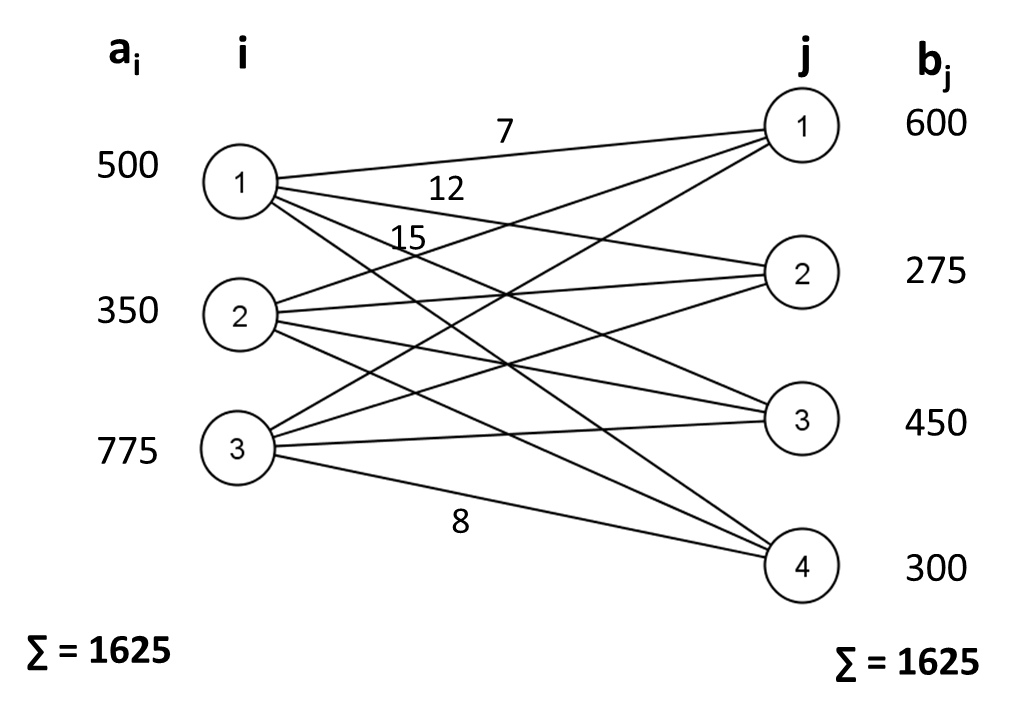
\includegraphics[scale=0.5]{Uebungen/figures/bipartiter_Graph_A_1}}
		\end{center}

		\uline{Model of the classic Transportation Problem}\\
	
			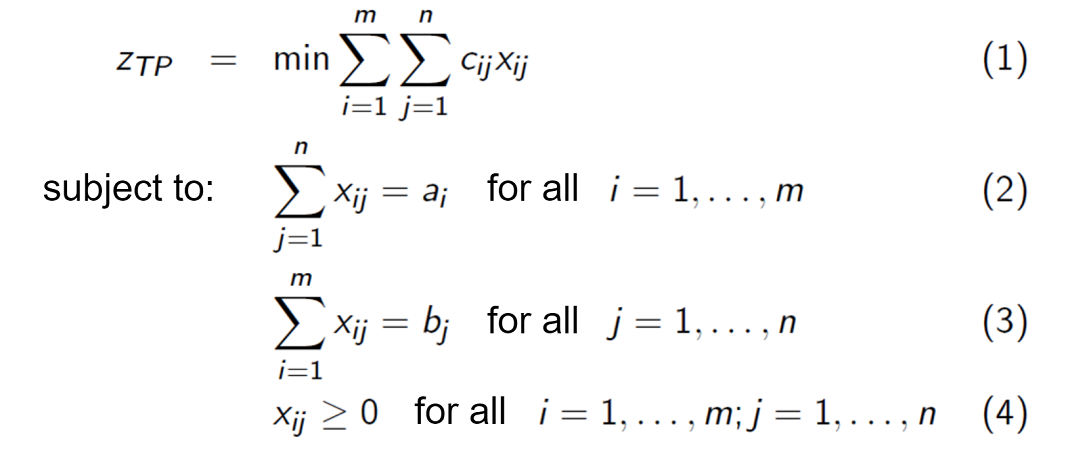
\includegraphics[scale=0.35]{Uebungen/figures/klassisches_TPe}\\

		\uline{Given case of the classical Transportation Problem}\\
		$min$ $z_{TP}= 7x_{11}+12x_{12}+15x_{13}+10x_{14}+16x_{21}+11x_{22}+6x_{23}+9x_{24}+14x_{31}+5x_{32}+17x_{33}+8x_{34}$\\
		s.t.\\
		\phantom{
		\begin{tabular}{ll}
			$i=1$& $x_{11}+x_{12}+x_{13}+x_{14}=500$\\
			$i=2$& $x_{21}+x_{22}+x_{23}+x_{24}=350$\\
			$i=3$& $x_{31}+x_{32}+x_{33}+x_{34}=775$\\
			&\\
			$j=1$& $x_{11}+x_{21}+x_{31}=600$\\
			$j=2$& $x_{12}+x_{22}+x_{32}=275$\\
			$j=3$& $x_{13}+x_{23}+x_{33}=450$\\
			$j=4$& $x_{14}+x_{24}+x_{34}=300$\\
		\end{tabular}}
		
		$x_{11}$, $x_{12}$, $x_{13}$, $x_{14}$, $x_{21}$, $x_{22}$, $x_{23}$, $x_{24}$, $x_{31}$, $x_{32}$, $x_{33}$, $x_{34}\geq 0$
	\end{solution}
	\item \label{a2} Determine an optimal transportation plan using the solver in Microsoft Excel! (See the following tutorial in \href{http://logistik.bwl.uni-mainz.de/373.php}{http://logistik.bwl.uni-mainz.de/373.php} under ``Microsoft Office").
	
	\begin{solution}
	The optimal transportation plan is:\\
	$x_{11}=500$, $x_{31}=100$, $x_{32}=275$, $x_{23}=350$, $x_{33}=100$, $x_{34}=300$\\
	The minimum total cost is 12,475.
	\end{solution}
	
	\item What happens if you run Solver the same way as in \ref{a2} but with total supply unequal to total demand?
	\begin{solution}
		An example, if $a_1=501$, then the supply exceeds the demand by one unit. Solver can no longer  find a feasible solution, since the constraint for suppliers $a_i$ cannot be simultaneously fulfilled.
	\end{solution}

% ----------------------------------
% Erweiterung mit ZIMPL/SCIP
% ----------------------------------

\item On Moodle you will find the file \texttt{transportproblem.zpl}. Open it with a text editor (e.g. Notepad). This is a model in Zimpl format. \\
\textbf{Note:} See the following tutorial in \href{http://logistik.bwl.uni-mainz.de/373.php}{http://logistik.bwl.uni-mainz.de/373.php} under ``SCIP/Zimpl".
\begin{enumerate}
	\item Complete the model using Zimpl notation (\url{https://zimpl.zib.de/download/zimpl.pdf}).
	\item Extend the model to include suppliers 4 and 5, who offer quantities $a_4=250$ and $a_5=100$, and customers 5, 6, and 7, who require quantities $b_5=50$, $b_6=150$, and $b_7=150$. This will result in the extended transportation cost matrix: \\
  \begin{center}
    \begin{tabular}{c|ccccccc}
    $c_{ij}$ & j=1   & j=2   & j=3   & j=4	& j=5	& j=6	& j=7 \\
    \hline
    i=1   & 7     & 12    & 15    & 10 		& 3			& 15		& 6\\
    i=2   & 16    & 11    & 6     & 9 		& 10		& 8			& 3\\
    i=3   & 14    & 5     & 17    & 8  		& 12		& 3			& 8\\
    i=4		& 4			& 13		& 16		& 5			& 14		&	4			& 10\\
    i=5		&	12		& 6			& 18		& 13		& 3			& 17		& 15\\	
    \end{tabular}
  \end{center}
	\item Compile the extended model (in Zimpl notation) and then solve with the Scip solver. Give the result.
	\begin{solution}
		The solution to the extended transportation problem is: $x_{11}=350$, $x_{17}=150$, $x_{23}=350$, $x_{32}=225$, $x_{33}=100$, $x_{34}=300$, $x_{36}=150$, $x_{41}=250$, $x_{52}=50$, $x_{55}=50$\\
		The minimum total cost is 12,575.
	\end{solution}
\end{enumerate}

% --------------------------------------------
% Alternativ Erweiterung mit Excel-Solver
% --------------------------------------------

%	\item Extend the model to include suppliers 4 and 5, who offer quantities $a_4=250$ and $a_5=100$, and customers 5, 6, and 7, who require quantities $b_5=50$, $b_6=150$, and $b_7=150$. This will result in the extended transportation cost matrix: \\
%  \begin{center}
%    \begin{tabular}{c|ccccccc}
%    $c_{ij}$ & j=1   & j=2   & j=3   & j=4	& j=5	& j=6	& j=7 \\
%    \hline
%    i=1   & 7     & 12    & 15    & 10 		& 3			& 15		& 6\\
%    i=2   & 16    & 11    & 6     & 9 		& 10		& 8			& 3\\
%    i=3   & 14    & 5     & 17    & 8  		& 12		& 3			& 8\\
%    i=4		& 4			& 13		& 16		& 5			& 14		&	4			& 10\\
%    i=5		&	12		& 6			& 18		& 13		& 3			& 17		& 15\\	
%    \end{tabular}
%  \end{center}
%	
%	\item Solve the extended model using the Microsoft Excel solver. Give the result.
%	\begin{solution}
%		The solution to the extended transportation problem is: $x_{11}=350$, $x_{17}=150$, $x_{23}=350$, $x_{32}=225$, $x_{33}=100$, $x_{34}=300$, $x_{36}=150$, $x_{41}=250$, $x_{52}=50$, $x_{55}=50$\\
%		The minimum total cost is 12,575.
%	\end{solution}
\end{enumerate}	

Now go back to the original model. The students quickly discover that an unexpected increase in demand at all four venues has almost used up their available beverage supply. The breweries are unable to meet the additional demand of 100 liters for each venue, needed quickly by the end of the test phase. Therefore, students are now questioning whether their transportation plan constructed in \ref{a2}. continues to be cost-minimal. Clearly, if there is excess demand, i.e. $\sum_{i=1}^{m} a_i < \sum_{j=1}^{n} b_j$, the restrictions on the event locations could alternatively be specified in inequality form instead of equality form, resulting in, for example, the following \emph{modified} TP:
	\begin{eqnarray}\setcounter{equation}{1}
	&&\min \sum_{i=1}^m\sum_{j=1}^n c_{ij} x_{ij} \label{TP1} \\
	\mbox{s.t.}&& \nonumber \\
	&&\sum_{j=1}^n x_{ij} = a_i \quad \forall i=1,\ldots,m \label{TP2}\\
	&&\sum_{i=1}^m x_{ij} \leq b_j \quad \forall j=1,\ldots,n \label{TP3}\\
	&&x_{ij} \geq 0\qquad \forall i=1,\ldots,m; j=1,\ldots,n \label{TP4}
	\end{eqnarray}
\begin{enumerate}
\setcounter{enumi}{4}
	\item What could you first change in the graph from \ref{a1}. to create a ``balance" between quantity offered and quantity demanded?
	\begin{solution}
	
	In the graph from 1. you could introduce a fictitious dummy supplier, which supplies the excess demand.
	\uline{}
		\begin{center}
			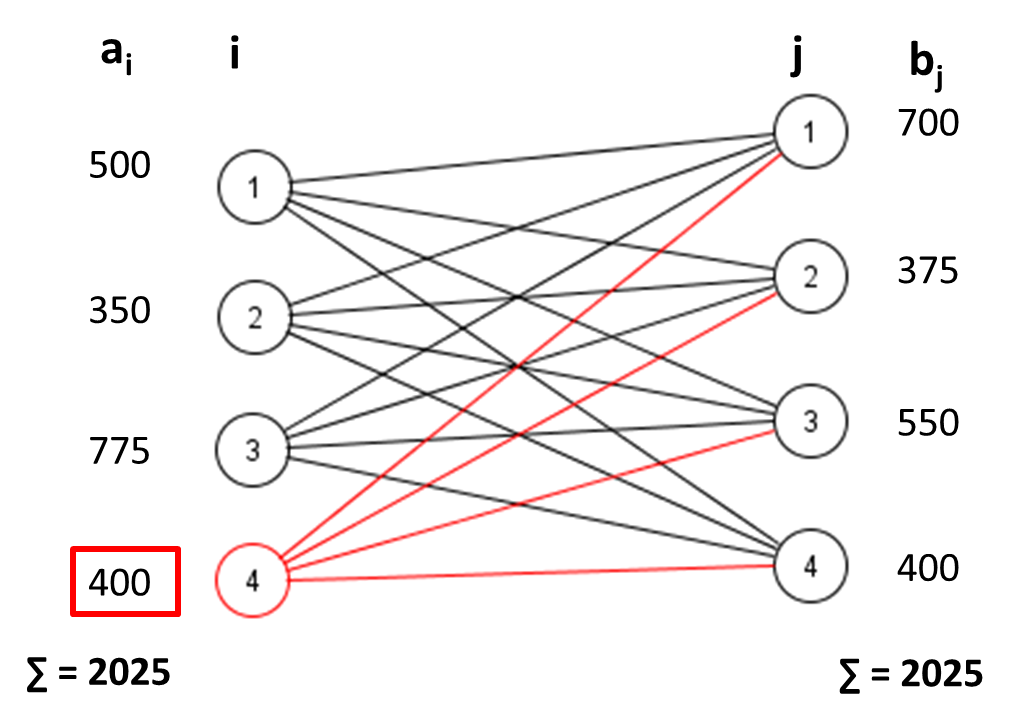
\includegraphics[scale=0.5]{Uebungen/figures/bipartiter_Graph_A_1_4}\\
		\end{center}
	\end{solution}
	\item \label{a5} Now transform the modified TP (\ref{TP1})-(\ref{TP4}) back into a classical TP! What information do the additional variables tell you?
	\begin{solution}
	
		\uline{Transformation of the modified Transportation Problem into a classical Transportation Problem}
		\begin{eqnarray}\setcounter{equation}{5}
			&&\min \sum_{i=1}^m\sum_{j=1}^n c_{ij} x_{ij}\phantom{+\red{\sum_{j=1}^n c_{m+1,j}x_{m+1,j}}} \\
			\mbox{s.t.}&& \nonumber \\
			&&\sum_{j=1}^n x_{ij} = a_i \quad \forall i=1,\ldots,\phantom{\red{m+1}} \\
			&&\sum_{i=1}^\red{\phantom{m+1}} x_{ij} = b_j \quad \forall j=1,\ldots,n \\
			&&x_{ij} \geq 0\qquad \forall i=1,\ldots,\phantom{\red{m+1}}; j=1,\ldots,n \\
	\end{eqnarray}
	\uline{Information from the additional variables}\\
	The additional variables $x_{m+1,1},\ldots, x_{m+1,n}$ distribute a fictitious supply $a_{m+1}$ to the real customers to compensate for the excess quantity of demand $\left(\sum_j b_j-\sum_i a_i\right)$.
	The values of the dummy variables in a (feasible or optimal) solution provide information about the so-called slack.\\
	$\Rightarrow$ Economic interpretation: The slack here indicates the degree of the demand shortfall.
	\end{solution}
	\item \label{6} Using a small an example, show how the modified TP (\ref{TP1})-(\ref{TP4}) can be transformed into the classical TP form!
	\begin{solution}
		Example:\\
		The modified TP:\\
				$min$ $z_{TP}= 1x_{11}+10x_{12}+10x_{21}+1x_{22}$\\
				s.t.\\
				$x_{11}+x_{12}=50$\\
				$x_{21}+x_{22}=50$\\
				
				$x_{11}+x_{21}\leq 55$\\
				$x_{12}+x_{22}\leq 55$\\
				
				$x_{11}$, $x_{12}$, $x_{21}$, $x_{22}\geq0$\\
				
		Feasible (optimal) solution of the modified TP:\\
		\begin{tabular}{c|cc|c}
		&$B_1$&$B_2$&$a_i$\\
		\hline
		$A_1$&50&0&50\\
		$A_2$&0&50&50\\
		\hline
		$b_j$&55&55&\\
		\end{tabular}
		
		$x_{11}=50$, $x_{12}=0$, $x_{21}=0$, $x_{22}=50$\\
		$z_{TP}= 1x_{11}+10x_{12}+10x_{21}+1x_{22}=1\cdot50+10\cdot0+10\cdot0+1\cdot50=100$\\
		
		
		The classic Transportation Problem:\\
		$min$ $z_{TP}= 1x_{11}+10x_{12}+10x_{21}+1x_{22}$\\
		s.t.\\
		$x_{11}+x_{12}=50$\\
		$x_{21}+x_{22}=50$\\
		\phantom{\red{$x_{31}+x_{32}=10$}}\\
		
		$x_{11}+x_{21}+\phantom{\red{x_{31}}}=55$\\
		$x_{12}+x_{22}+\phantom{\red{x_{32}}}=55$\\
		
		$x_{11}$, $x_{12}$, $x_{21}$, $x_{22}$,$\phantom{\red{x_{31}}}$, $\phantom{\red{x_{32}}} geq0$\\
		
		Note: The cost coefficients of the dummies are all chosen to be equal to $0$.\\
		
		Feasible (optimal) solution of the classical TP:\\
		\begin{tabular}{c|cc|c}
			&$B_1$&$B_2$&$a_i$\\
			\hline
			$A_1$&50&0&50\\
			$A_2$&0&50&50\\
			$\red{D}$&\phantom{\red{5}}&\phantom{\red{5}}&\phantom{\red{0}}\\
			\hline
			$b_j$&55&55&\\
		\end{tabular}
	\end{solution}		
		
	\item \label{7} Bonus: What happens when the cost of the dummy variables are chosen to be nonzero in the transition from the modified to the classical Transportation Problem?
		
	\begin{solution}
		1st possibility: The cost coefficients of the dummies are all chosen to be the same.\\
			$min$ $z_{TP}= 1x_{11}+10x_{12}+10x_{21}+1x_{22}+\phantom{\red{10x_{31}+10x_{32}}}$\\
				s.t.\\
				$x_{11}+x_{12}=50$\\
				$x_{21}+x_{22}=50$\\
				\red{$x_{31}+x_{32}=10$}\\
				
				$x_{11}+x_{21}+\red{x_{31}}=55$\\
				$x_{12}+x_{22}+\red{x_{32}}=55$\\
				
				$x_{11}$, $x_{12}$, $x_{21}$, $x_{22}$, $\red{x_{31}}$, $\red{x_{32}}\geq0$\\
				
		Feasible (optimal) solution of the classical TP:\\
		\begin{tabular}{c|cc|c}
		&$B_1$&$B_2$&$a_i$\\
		\hline
		$A_1$&50&0&50\\
		$A_2$&0&50&50\\
		$\red{D}$&\red{5}&\red{5}&\red{10}\\
		\hline
		$b_j$&55&55&\\
		\end{tabular}
		
		$x_{11}=50$, $x_{12}=0$, $x_{21}=0$, $x_{22}=50$, $x_{31}=5$, $x_{32}=5$\\
		$z_{TP}= 1x_{11}+10x_{12}+10x_{21}+1x_{22}+10x_{31}+10x_{32}=1\cdot50+10\cdot0+10\cdot0+1\cdot50+10\cdot5+10\cdot5=200$\\
		
		2nd possibility: The cost coefficients of the dummies are different.\\
			$min$ $z_{TP}= 1x_{11}+10x_{12}+10x_{21}+1x_{22}+\red{10x_{31}+20x_{32}}$\\
				s.t.\\
				$x_{11}+x_{12}=50$\\
				$x_{21}+x_{22}=50$\\
				\red{$x_{31}+x_{32}=10$}\\
				
				$x_{11}+x_{21}+\red{x_{31}}=55$\\
				$x_{12}+x_{22}+\red{x_{32}}=55$\\
				
				$x_{11}$, $x_{12}$, $x_{21}$, $x_{22}$, $\red{x_{31}}$, $\red{x_{32}}\geq0$\\
				
		Feasible (optimal) solution of the classical TP:\\
		\begin{tabular}{c|cc|c}
		&$B_1$&$B_2$&$a_i$\\
		\hline
		$A_1$&45&5&50\\
		$A_2$&0&50&50\\
		$\red{D}$&\red{10}&\red{0}&\red{10}\\
		\hline
		$b_j$&55&55&\\
		\end{tabular}
		
		$x_{11}=45$, $x_{12}=5$, $x_{21}=0$, $x_{22}=50$, $x_{31}=10$, $x_{32}=0$\\
		$z_{TP}= 1x_{11}+10x_{12}+10x_{21}+1x_{22}+10x_{31}+10x_{32}=1\cdot45+10\cdot5+10\cdot0+1\cdot50+10\cdot10+10\cdot0=245$\\
		
		As can be seen from the example, if the cost coefficients of the dummies are all the same, the optimal solutions of the model (\ref{TP1})-(\ref{TP4}) are transformed into the optimal solutions of the model in \ref{a5}. .
		
		In addition, the respective objective function values are exactly the same when the cost coefficient $\red{c}$ of the dummies is set equal to 0.\\
		
		Objective function of the classical Transportation Problem assuming equal cost coefficients of the dummies:\\
		$\sum_{i=1}^m\sum_{j=1}^n c_{ij} x_{ij}+\sum_{j=1}^n \red{c}x_{m+1,j}$\\
		Objective function of the modified Transportation Problem:\\.
		$\sum_{i=1}^m\sum_{j=1}^n c_{ij} x_{ij}$\\.
		
		For these two objective function values to be equal, it must hold:\\
 		
 		 $\sum_{i=1}^m\sum_{j=1}^n c_{ij} x_{ij}+\sum_{j=1}^n \red{c}x_{m+1,j}=\sum_{i=1}^m\sum_{j=1}^n c_{ij} x_{ij}$ $\Leftrightarrow$\\
 		 $\sum_{j=1}^n \red{c}x_{m+1,j}=0$ $\Leftrightarrow$\\
 		 $\red{c} \sum_{j=1}^n x_{m+1,j}=0$ \\
 		
 		 Since $\sum_{j=1}^n x_{m+1,j}=\sum_{j=1}^n b_j-\sum_{i=1}^m a_i = a_{m+1}\neq 0$, then $\red{c}=0$ must hold so that the objective function values are equal.
 		
 		 Note:
 		 If $c>0$ then the $x_{ij}^*$ are identical, but the objective function values will differ.
	\end{solution}	
\end{enumerate}